This section is concerned with the control structure of the WDN. 
\subsection{Control Structure}
This section documents the structure of the control system for this project as seen in \cref{fig:controlstructure}. The intended control structure assumes that the dynamics of the system can be partitioned in two, the fast dynamics of the inertia of the pipes (assuming the pump dynamics are infinitely fast) and the slow dynamics of the tank level.
\begin{figure}[!htb] 
	
	
	\centering
	\begin{tikzpicture}[auto, node distance=2.5cm,>=latex']
		% ========================== Nodes ============================
		% Nodes in upper vertical line
		\node [input, name=rinput] (rinput) {};
		\node [sum, right of=rinput] (sum1) {};
		\node [block, right of=sum1, node distance = 1.5cm] (LQR) {LQR};
		\node [sum, right of=LQR, node distance =
		1.5cm] (sum2) {};
		\node [block, right of=sum2, node distance = 1.5cm] (PI){PI};
		\node [block, right of=PI, align=center] (Fast){Fast\\Dynamics};
		\node [block, right of=Fast, node distance = 3cm, align=center] (Slow){Slow\\Dynamics};
		\node [output, right of=Slow] (output) {};
		
		% Nodes for inner feedback
		\node [tmp, right of=Fast, node distance = 1.5cm] (tmp0){};
		\node [tmp, below of=tmp0, node distance = 1.5cm] (tmp1){};
		\node [tmp, below of=sum2, node distance = 1.5cm] (tmp2){};
		
		% Nodes for outer feedback
		\node [tmp, right of=Slow, node distance = 1.5cm] (tmp10){};
		\node [tmp, below of=tmp10,node distance = 2.5cm] (tmp11){};
		\node [tmp, below of=sum1, node distance = 2.5cm] (tmp12){};
		
		% Nodes for Disturbance
		\node [tmp, above of=tmp0, node distance = 2.5cm] (tmp20){};
		\node [tmp, above of=tmp0, node distance = 2cm] (tmp21){};
		\node [tmp, above of=Fast, node distance = 2cm] (tmp22){};
		\node [tmp, above of=Slow, node distance = 2cm] (tmp23){};
		
		\draw[thick, dotted] ($(Fast.north west)+(-0.25, 0.25)$) rectangle  ($(Slow.south east)+(0.25, -0.25)$);
		\node[above of =tmp0, node distance =1.1cm](sys_txt) {System};
		
		% ========================== Lines ============================
		
		% Lines in upper vertical part of block diagram
		\draw [->] (rinput) -- node{$p_{ref}$} (sum1);
		\draw [->] (sum1) --node[name=z,anchor=north]{} (LQR);
		\draw [->] (LQR) -- node{$ q_{ref} $}(sum2);
		\draw [->] (sum2) -- (PI);
		\draw [->] (PI) -- node[pos=0.4]{$ \omega_{ref} $}(Fast);
		\draw [->] (Fast) -- node{$d_p$}(Slow);
		\draw [->] (Slow) -- node{$p_{\tau}$}(output);	
		
		% Lines for inner feedback
		\draw [-] (tmp0) -- (tmp1);
		\draw [-] (tmp1) -- (tmp2);
		\draw [->] (tmp2) -- node[pos=0.99]{$ - $}(sum2);
		
		
		% Lines for outer feedback
		\draw [-] (tmp10) -- (tmp11);
		\draw [-] (tmp11) -- (tmp12);
		\draw [->] (tmp12) -- node[pos=0.99]{$ - $}(sum1);
		
		
		% Lines for disturbance
		\draw [-] (tmp20)node[above, align=center]{Consumer \\ Disturbance} -- (tmp21);
		\draw [-] (tmp21) -- (tmp22);
		\draw [-] (tmp21) -- (tmp23);
		\draw [->] (tmp22) -- node[left, pos = 0.5]{OD}(Fast);
		\draw [->] (tmp23) -- node[pos = 0.5]{$ d_c $}(Slow);
		
		
	\end{tikzpicture}
	\caption{Control Structure} \label{fig:controlstructure}
\end{figure}


\subsection{System Linearisation}\label{subsec:Linearisation}

Before the model presented in \cref{eq:NonLinearModelWithTank} is truly useful to us - at least within the scope of the \textit{linear} control strategies considered in this project - we must find a way to turn it into a linear model. The typical approach to this problem is \textit{linearisation}, whereby we exploit the extremely powerful Hartman-Grobman theorem, which we present roughly as outlined in \cite{Perko2001}:


\begin{theorem}\label{theorem:HartmanGrobman}
(\textbf{The Hartman-Grobman Theorem}) Let $E$ be an open subset of $\mathbb{R}^n$ containing the origin, and let $f$ be a continuously differentiable function on $E$:
 
\begin{equation*}
f \in C^1(E)
\end{equation*}

Let $\gamma_t$ be the flow of the nonlinear system $\dot{x} = f(x)$. Assume furthermore that there exists an equilibrium point at the origin: 

\begin{equation*}
f(0) = 0
\end{equation*}

and that this equilibrium point is hyberbolic: 

\begin{equation*}
\forall \lambda \in T(A): \ \text{Re}(\lambda) \neq 0, \quad A = \nabla f  
\end{equation*}

where $T$ is the eigenspace of $A$. Then there exists a homeomorphism $H$ of some open set $U, \ 0 \in U$ onto the open set $V, \ 0 \in V$, such that $\forall x_0 \in U$, there is an open interval $I_0 \subset \mathbb{R}, \ 0 \in I_0$ such that:

\begin{equation*}
	\forall x_0 \in U \wedge \forall t \in I_0: \ H \circ \gamma_t(x_0) = e^{At}H(x_0)
\end{equation*}
\end{theorem}

At first glance, this theorem looks opaquely mathematical and not immediately applicable. However, in practice, \cref{theorem:HartmanGrobman} simply tells us that in the immediate vicinity of some hyperbolic equilibrium point of our non-linear system, there exists a \textit{linear} system whose eigenfunctions describe its evolution exactly. We note that it is not \textit{necessary} to linearise at a hyperbolic equilibrium, but doing so is favourable when possible as it precludes the presence of a center manifold, whose dynamics cannot be captured by linearisation.

Recalling that the first-order Taylor series of a function at a point can be thought of as a  generalisation of its tangent line, it is then possible to identify the linearisation of our system via:

\begin{equation}\label{eq:TaylorSeries}
\dot{x} \approx f(x_0) + \nabla f\bigg\rvert_{x_0} (x-x_0)
\end{equation}

We now revert our attention to the non-linear model of the WDN. We will make the simplifying assumption that $\Phi \mathcal{J} \Phi^T$ is invertible, which is not generally true, but tends to hold for the type of WDN in question. We also introduce the notation $\mathcal{P}: (\Phi \mathcal{J} \Phi^T)^{-1}$, allowing allows us to rewrite \cref{eq:NonLinearModelWithTank} as:

\begin{equation}\label{eq:NonLinearModelSimplified}
	\begin{split}
		\dot{q}_n &=  -\mathcal{P}\Phi\Big(\lambda(q_n)+\mu(q_n,OD)+\alpha(q_n,\omega)\Big) + \mathcal{P}\Big(\Psi(\bar{h}-\mathbf{1}h_0) + \mathcal{I}(p_{\tau}-\mathbf{1}p_0)\Big) \\
		&= 	-\mathcal{P}\Phi\Big(\lambda(q_n)+\frac{|q_n|q_n}{(K_v\cdot OD)^2}+\alpha(q_n,\omega)\Big) + 	\mathcal{P}\Big(\Psi(\bar{h}-\mathbf{1}h_0) + \mathcal{I}(p_{\tau}-\mathbf{1}p_0)\Big) \\
		& = -\mathcal{P}\Phi\Big(K_\lambda|q_n|q_n+\frac{|q_n|q_n}{(K_v\cdot OD)^2}+a_0\omega^2+a_1\omega q+a_2|q|q\Big) + \mathcal{P}\Big(\Psi(\bar{h}-\mathbf{1}h_0) + \mathcal{I}(p_{\tau}-\mathbf{1}p_0)\Big)
	\end{split}	
\end{equation}

We now make the additional observation that $\Psi(\bar{h}-\mathbf{1}h_0)$ does not depend on $\{q_n,OD,\omega,p_\tau\}$. This suggests that, when computing the Taylor expansion, this term disappears under the action of the $\nabla$ operator, i.e. that:

\begin{equation}\label{eq:PressureHeightDisappear}
	\begin{split}
		\nabla \dot{q}_n &= \nabla \Big(-\mathcal{P}\Phi\Big(\lambda(q_n)+\mu(q_n,OD)+\alpha(q_n,\omega)\Big) + \mathcal{P}\Big(\Psi(\bar{h}-\mathbf{1}h_0) + \mathcal{I}(p_{\tau}-\mathbf{1}p_0)\Big) \\ 
		&=\nabla \Big(-\mathcal{P}\Phi\Big(\lambda(q_n)+\mu(q_n,OD)+\alpha(q_n,\omega)\Big)\Big) + \nabla \mathcal{P}\Big({I}(p_{\tau}-\mathbf{1}p_0)\Big) \\
		&=\nabla \Big(-\mathcal{P}\Phi\Big(K_\lambda|q_n|q_n+\frac{|q_n|q_n}{(K_v\cdot OD)^2}+a_0\omega^2+a_1\omega q+a_2|q|q\Big)\Big) + \nabla \mathcal{P}\Big({I}(p_{\tau}-\mathbf{1}p_0)\Big)
	\end{split}
\end{equation}

Recognizing furthermore that $\Phi$ and $\mathcal{J}$ are simply linear transformations, the linearity of differentiation then allows us to write a general expression for the Taylor expansion of \cref{eq:NonLinearModelSimplified} as:

\begin{equation}\label{eq:SymbolicLinearisation}
	\begin{split}
		\dot{q}_n &\approx f(x_0) + \frac{\partial f}{\partial q_n}\bigg\rvert_{x_0} \tilde{q}_n + \frac{\partial f}{\partial OD}\bigg\rvert_{x_0} \tilde{OD} + \frac{\partial f}{\partial \omega}\bigg\rvert_{x_0} \tilde{\omega} +  \frac{\partial f}{\partial p_\tau}\bigg\rvert_{x_0} \tilde{p}_\tau
		\\
		&= f(x_0) + \mathcal{P}\Big(-\Phi\Big( \frac{\partial \Omega}{\partial q_n}\bigg\rvert_{x_0} \tilde{q}_n + \frac{\partial \Omega}{\partial OD}\bigg\rvert_{x_0} \tilde{OD} + \frac{\partial \Omega}{\partial \omega}\bigg\rvert_{x_0} \tilde{\omega} \Big) + \mathcal{I} \frac{\partial f}{\partial p_\tau}\bigg\rvert_{x_0} \tilde{p}_\tau \Big)
	\end{split}
\end{equation}

where: 

\begin{align}
	x_0 &= \{q_0,OD_0,\omega_0, p_\tau \} \label{eq:EquilibriumPoint} \\
	\Omega &= K_\lambda|q_n|q_n+\frac{|q_n|q_n}{(K_v\cdot OD)^2}+a_0\omega^2+a_1\omega q_n+a_2|q_n|q_n \label{eq:OmegaFun} \\
	\tilde{q}_n &= q_n - q_0 \label{eq:QTilde} \\
	\tilde{OD} &= OD - OD_0 \label{eq:ODTilde} \\ 
	\tilde{\omega} &= \omega - \omega_0 \label{eq:OmegaTilde} \\
	\tilde{p}_\tau &= p_\tau - p_{\tau_0}
\end{align}

Writing out each of the partial derivatives in \cref{eq:SymbolicLinearisation}, we get:

\begin{equation}\label{eq:PartialTaylorQ}
	\frac{\partial \Omega}{\partial q_n}\bigg\rvert_{x_0} 
	=
	a_1\omega_0 + \Big(|q_0|+ \text{sign}(q_0)q_0\Big)\Bigg(K_\lambda + a_2 + \frac{1}{(K_v OD_0)^2}\Bigg) 
\end{equation}

\begin{equation}\label{eq:PartialTaylorOD}
	\frac{\partial \Omega}{\partial OD}\bigg\rvert_{x_0} 
	=
	-|q_0|q_0 \frac{2}{K_v^2 OD_0^3}
\end{equation}

\begin{equation}\label{eq:PartialTaylorOmega}
	\frac{\partial \Omega}{\partial \omega}\bigg\rvert_{x_0} 
	=
	a_1 q_0 + 2a_0\omega_0
\end{equation}

\begin{equation}\label{eq:PartialTaylorPressure}
		\frac{\partial \Omega}{\partial p_\tau}\bigg\rvert_{x_0} 
	=
	1
\end{equation}

and the complete Taylor expansion becomes:

\begin{equation}\label{eq:SymbolicLinearisationExpanded}
	\begin{split}
			\dot{q}_n \approx f(x_0) &-\mathcal{P}\Phi\Bigg(a_1\omega_0 + \Big(|q_0|+\text{sign}(q_0)q_0\Big)\Bigg(K_\lambda + a_2 + \frac{1}{(K_v OD_0)^2}\Bigg) \tilde{q}_n \Bigg)  \\
			&- \mathcal{P}\Phi\Bigg(\Big(-|q_0|q_0 \frac{2}{K_v^2 OD_0^3}\Big) \tilde{OD}\Bigg) \\
			&-  \mathcal{P}\Phi\Bigg(\Big(a_1 q_0 + 2a_0\omega_0\Big) \tilde{\omega}\Bigg) \\
			&+ \mathcal{P} \mathcal{I} \tilde{p}_\tau
	\end{split}
\end{equation}

We will now make three additional abstractions to simplify \cref{eq:SymbolicLinearisationExpanded}. We first exploit the trivial condition that, when linearizing at an equilibrium point, $f(x_0) \equiv 0$. We then consider the fact that, in practice, $OD$ and $p_\tau$ vary very slowly compared to $q_n$ and $\omega$. It is therefore a reasonable assumption that at steady state for the latter variables, the error introduced by neglecting $\frac{\partial\Omega}{\partial OD}$ is:

\begin{equation}\label{eq:IgnoreODError}
	\mathcal{P}\Phi\Big(|\tilde{q}_{ss}|\tilde{q}_{ss}\frac{2}{K_v^2 OD_0^3} \tilde{OD}\Big)
\end{equation}

which, under the assumption that $q_n$ changes much faster than $OD$, is a constant offset and therefore removable by integral action. Analogously, the error induced by ignoring $\frac{\partial\Omega}{\partial p_\tau}$ is: 

\begin{equation}\label{eq:IgnorePressureError}
	\mathcal{P}\mathcal{I}\tilde{p}_\tau
\end{equation}

which is likewise a constant term that may be removed by integral action. Thus, we can restate a greatly simplified form of \cref{eq:SymbolicLinearisationExpanded} as:

\begin{equation}\label{eq:SymbolicLinearisationSimplified}
	\dot{q}_n \approx -\mathcal{P}\Phi\Bigg(a_1\omega_0 + \Big(|q_0|+\text{sign}(q_0)q_0\Big)\Bigg(K_\lambda + a_2 + \frac{1}{(K_v OD_0)^2}\Bigg) \tilde{q}_n \Bigg) -  \mathcal{P}\Phi\Bigg(\Big(a_1 q_0 + 2a_0\omega_0\Big) \tilde{\omega}\Bigg)
\end{equation}

\subsection{Linearised Model} \label{sec:LinearisedModel}
In the following section state space models are presented both for the fast and the slow system, i.e. the pump flow and the tank pressure dynamics respectively. 

\subsubsection{State Space Model - Pump Dynamics}
Before linearising the system model, presented in \cref{eq:NonLinearModelWithTank}, we need to identify the equilibrium points. This is done by evaluating the model at fixed $ \omega $ and $ OD $, with its dynamics set to $0$. We choose pump speeds as an average of those used in \cref{ap:PumpCoef}, which is $ 66\% $ for each pump. We set $ OD $ to $ 0.5 $ for each valve. This yields the following equilibrium point:

	\begin{equation}
	q_c^* = \kbordermatrix{
		\\
		q_3 & 0.1992 \\ 
		q_7 & 0.0231\\
	}
\end{equation}
	\begin{equation}
	\bar{d}_f^* = \kbordermatrix{
		\\
		d_1 & 0.3752 \\ 
		d_5 & -0.2913\\
		q_9 & -0.2876\\
	}
	\end{equation}

\begin{equation}
	d_\tau^* = 0
\end{equation}


The linearised model of the system can then be expressed on the standard state space form given in \cref{eq:StateSpace} by evaluating \cref{eq:SymbolicLinearisationSimplified} at the equilibrium point: 

\begin{equation}\label{eq:StateSpace}
	\begin{split}
	\dot{x} = Ax + Bu \\
	y = Cx
	\end{split}
\end{equation}

\begin{equation}
	A = \begin{bmatrix}
		-0.3236 & -0.0406 & -0.1577 & 10.0671 & -0.7623 & 0.0000\\
		-0.1429 & -0.3189 & 0.2176 & -1.3489 & -6.0984  & 0\\
		-0.0275 & 0.0687 & -0.3968 & 7.1758 & 1.5246 & 0\\
		0.1089 & 0.0687 & 0.0196 & -20.2792 & 1.5246 & -0.0000\\
		-0.0551 & -0.0443 & -0.0272 & 1.4425 & -15.3466 &   -0.0999\\
		0.1486 & 0.0817 & -0.2877 & 11.1436 & 8.2419 & -0.4174\\
	\end{bmatrix}
\end{equation}

\begin{equation}
	B = \begin{bmatrix}
		0.0982 & 0.0000\\
		0.0078 & 0 \\
		0.1147 & 0 \\
		-0.0408 & 0 \\
		-0.0087 & -0.0193\\
		-0.0651 & -0.0715
	\end{bmatrix}
\end{equation}

The output matrix $ C $ is then constructed to extract the pump flows from the states of the system:

\begin{equation}
C =	\begin{bmatrix}
	&0&0&1&0&0&0\\
	&0&0&-1&-1&-1&-1\\	
\end{bmatrix} 
\end{equation}

This yields a system with pump speeds $ \{\omega_1 , \omega_2 \} $ as inputs and pump flows $ \{d_1, d_{13}\} $ as outputs:

\begin{equation}\label{eq:StateSpaceInputsOutputsFast}
	\begin{split}
		u = \begin{bmatrix} \omega_1 \\ \omega_2	\end{bmatrix} \\
		x = \begin{bmatrix} q_c \\ d_f \\ d_{\tau}	\end{bmatrix} \\
		y = \begin{bmatrix} d_1 \\ d_{13} \\ 	\end{bmatrix} \\
	\end{split}
\end{equation}

\subsubsection{State Space Model - Tank Pressure Dynamics}
The tank pressure dynamics are significantly simpler than the fast dynamics of the system - in fact, the slow tank pressure dynamics of the system are a linear first-order system that, per \cref{eq:TankDynamics}, evolve according to:

\begin{equation}\label{eq:SlowTankDynamics}
	\begin{split}
		\dot{p}_\tau &= - \tau d_\tau \\
		&= \tau \left(d_1 + d_{13} + d_5 + d_9\right)
	\end{split}
\end{equation}

We can discretise this with Euler's method, resulting in:

\begin{equation}\label{eq:TankDynamicsDiscrete}
	\begin{gathered}
			p_\tau(k+1) = p_\tau(k) + \tau \left(d_1(k) + d_{13}(k) + d_5(k) + d_9(k)\right)t_s = \mathcal{T}\left(d_1(k) + d_{13}(k) + d_5(k) + d_9(k)\right) \\ 
			\mathcal{T} = \tau\cdot t_s 
	\end{gathered}
\end{equation}

which can be converted into the following state-space system:

\begin{equation}\label{eq:TankPressureStateSpace}
	\begin{gathered}
				p_\tau(k+1) = A p_\tau(k) + B_pd_p(k) + B_cd_c(k)
				= A p_\tau(k) + \left(B_p \begin{bmatrix}d_1(k) \\ d_{13}(k)\end{bmatrix} 
				+ B_c\begin{bmatrix}d_5(k) \\ d_9(k)\end{bmatrix}\right) \\      
				A = 1, \ B_p = \begin{bmatrix} \mathcal{T} & \mathcal{T} \end{bmatrix}, \ B_c = \begin{bmatrix} \mathcal{T} & \mathcal{T} \end{bmatrix}
	\end{gathered}
\end{equation}

We note the presence of $B_cd_c$, an exogenous input over which we have no control. This will be addressed in \cref{sec:LQR,sec:KalmanFilter}.

\subsection{Influence of Pump Delay}
The pumps of the WDN system introduces a delay of approximately 4 seconds. According to \cite[pp. 182-183]{Skogestad2005}, 
a time delay $\theta$ limits the feasible closed-loop bandwidth of a system to:

\begin{equation}\label{eq:BWdelay}
	\omega_c < \frac{1}{\theta}
\end{equation}

This limitation on the inner loop inherently limits the outer loop as well, so long as standard cascade control practices are observed. Typically, the inner loop is required to be at least $5$ times faster than the outer loop.


\clearpage

\subsection{The Root Locus Method}

For design of the pump controllers the root locus method will be used. The root locus is a powerful visual tool that investigates the location of the closed-loop poles of a system, when introducing feedback with a gain $K$. The root locus can be drawn by hand by calculating the location of the closed-loop poles of a system for a large number of feedback gains. In practice however, this is done using a software package like Matlab.

While there exist many rules for sketching root locus by hand, only a few of them are truly important to understand how the root locus is used for controller design:

\begin{enumerate}
	\item The closed-loop poles of the system move from the open-loop poles at $ K=0 $ to the open-loop zeros as $K \to \infty$, unless the number of poles and zeros is different, in which case the closed-loop poles will go to or come in from infinity.
	\item The number of lines going to or from $\infty$ is equal to the difference between the number of open-loop poles and zeros.
	\item The angle and place of gravity of the lines going to or from $ \infty $ is dependent of the difference between the number of open-loop poles and zeros and their location in the complex plane.
\end{enumerate}

The first part of rule $1$ tells us that the closed-loop poles are equal to the open-loop poles when $ K=0 $. This is intuitively understood as $ K=0 $ means there is no feedback, thus the closed and open-loop systems are identical. The second part tells us that when $K \to \infty$ the closed-loop poles will be located at the open-loop zeros. This is understood by analysing the closed-loop transfer function when the open-loop transfer function is given as
\begin{equation}
	G_{ol}(s) = \frac{Z(s)}{P(s)}
\end{equation}

where Z(s) and P(s) are the polynomials describing the zeros and poles respectively.
The closed-loop transfer function is thus
\begin{equation}
	G_{cl}(s) = \frac{G_{ol}(s)}{1 + K G_{ol}(s)}
\end{equation}

where the roots are the values of s that make the denominator equal to 0

\begin{equation}
	0 = 1 + K \cdot G_{ol}(s) = 1 + K \frac{Z(s)}{P(s)}
\end{equation}

Restructuring this yields

\begin{equation}
	0 = 1 + K \frac{Z(s)}{P(s)} = 1P(s) + K \frac{Z(s) P(s)}{P(s)} = P(s) + K Z(s)
\end{equation}

This confirms that setting $ K=0 $ makes the closed-loop poles equal to P(s) which is exactly the open-loop poles. When $K \to \infty$ the $ KZ(s) $ term is dominating, which is why the closed-loop poles will then equal the open-loop zeros $ Z(s) $.

Rules $2$ and $3$ simply tells us that the possible locations of the closed-loop poles - specified by the loci - changes with the position of the open-loop poles and zeros. This enables the designer to place additional poles and zeros to change the behaviour of the closed-loop system. 


\subsection{Design of Pump Controllers}
This section will cover design of the inner-loop pump controllers, which corresponds to control of the fast dynamics of the system.

\subsubsection{Decentralised Control}
Based on the obtained linearised model, controllers for the pumps are being introduced. Its desired to obtain decentralised control as this mitigates network faults and decrease delays in the system. Decentralised control can be obtained in a MIMO system if the plant is close to diagonal, meaning that the system can be considered a collection of independent sub-systems \cite[p. 91]{Skogestad2005}. 
In order to validate whether decentralised control can be obtained, the interactions in the off-diagonals of the system are investigated with magnitude plots. For this analysis the tank is assumed to have a constant pressure. This is part of the separation of the inner and outer loop, where the outer loop is assumed to be slow enough to be ignored in analysis of the inner loop. The magnitude plots can be seen in \cref{fig:PumpMagPlot}. They show the gain from a input frequency $\omega$ on each of the pumps to the output flows of the pumps.

\begin{figure}[h!]
	\centering
		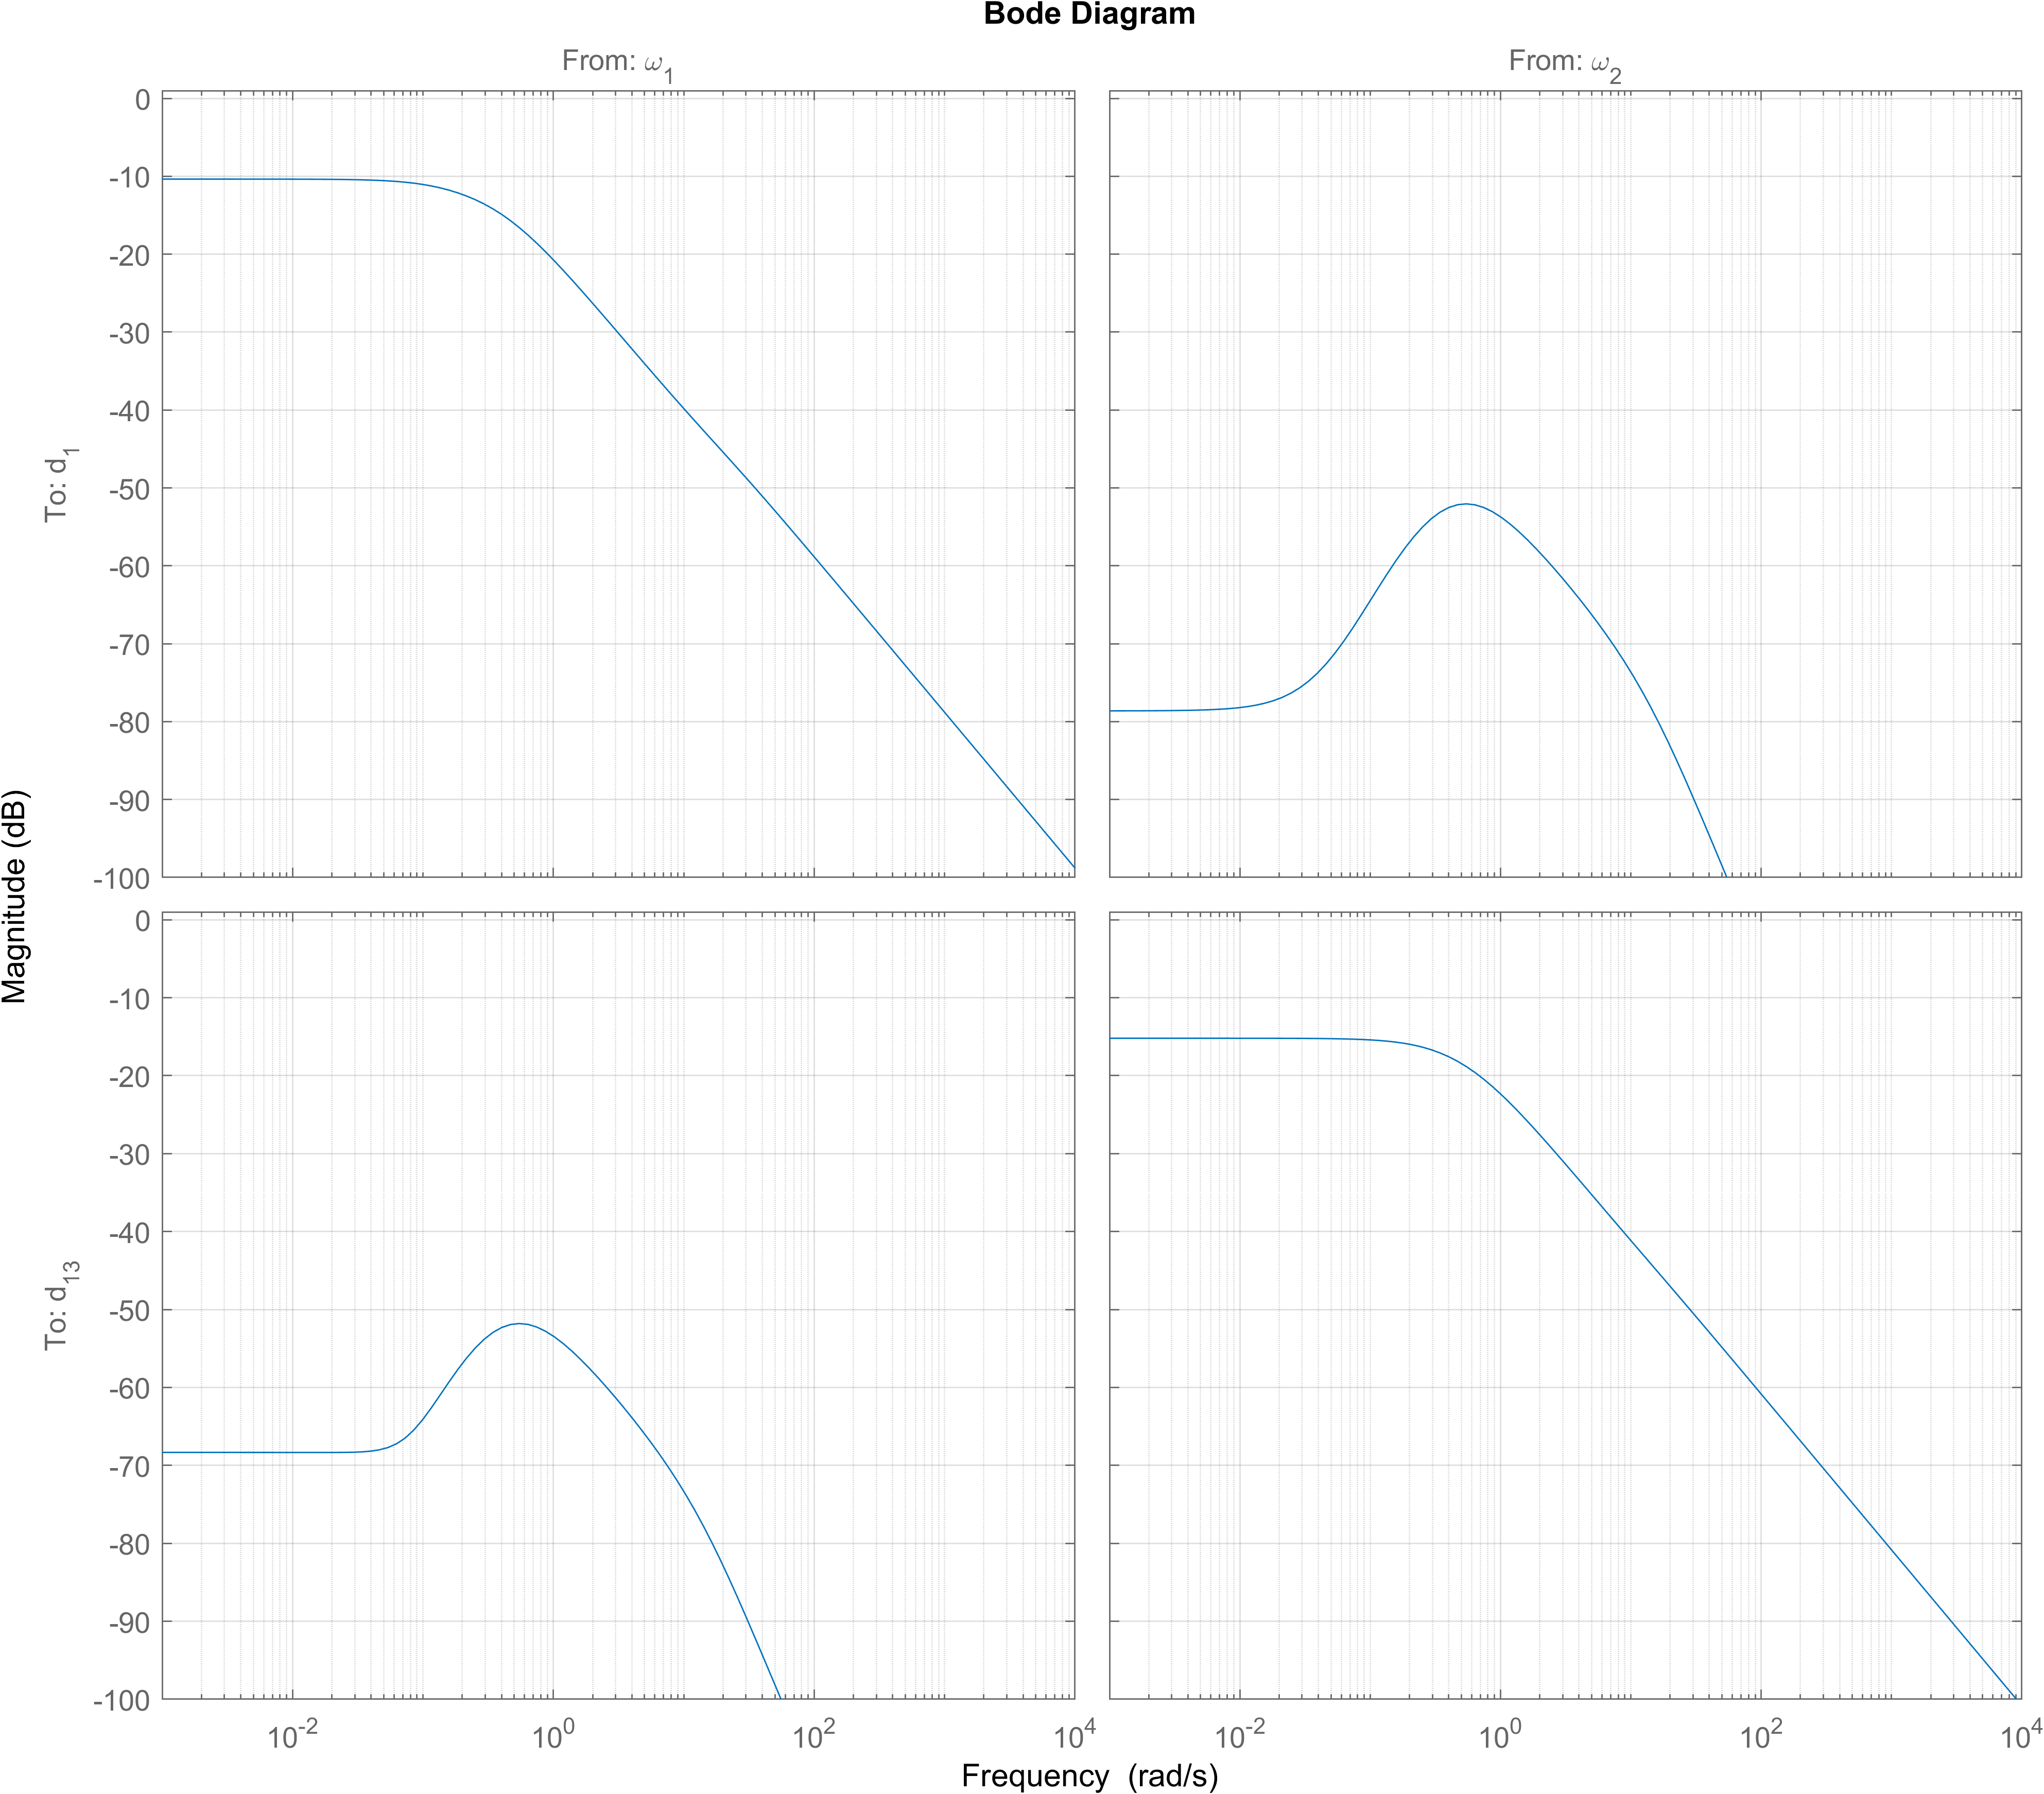
\includegraphics[width=0.8\textwidth]{Pictures/PumpMagPlot.png}
		
		\caption{Magnitude Plot from inputs to outputs}
	\label{fig:PumpMagPlot}
\end{figure}

As seen in \cref{fig:PumpMagPlot}, the gain from $\omega_1$ to $d_{13}$ is for all frequencies less than $ -50 \ \si{dB} $, compared to $ -10 \ \si{dB} $ from $\omega_1$ to $d_1$. \\
Likewise, the gain from $\omega_2$ to $d_1$ is less than $ -50 \ \si{dB} $ for all frequencies, compared to $ -15 \ \si{dB} $ from $\omega_2$ to $d_{13}$.\\
In both cases, the coupling is at least $ -35 \ \si{dB} $ corresponding to less than a factor of $ \frac{1}{50} $, and the system can reasonably be assumed to have no meaningful cross-coupling, which allows for independent SISO design of the respective controllers solely from the diagonal transfer functions in the transfer matrix.

\subsubsection{Model Order Reduction}
On closer comparison, the diagonal transfer functions can be seen to have approximately identical poles and zeroes in  \cref{eq:PumpDiagonalPolesZeros}: 

\begin{equation}\label{eq:PumpDiagonalPolesZeros}
	\begin{gathered}
		z_{11} = \begin{bmatrix}-18.9173&  -13.9942&   -0.5571&   -0.3357&   -0.1944 \end{bmatrix} \\
		z_{22} = \begin{bmatrix}-20.7216&  -14.1600&   -0.4079&   -0.3639&   -0.1597 \end{bmatrix} \\
		p_{11} = p_{22} = \begin{bmatrix} 20.7703&  -14.8635&   -0.5624&   -0.3930&   -0.3337&   -0.1597 \end{bmatrix} \\
	\end{gathered}
\end{equation}

Realising that many of the poles more or less cancel out with the zeros can simplify the model significantly for the root locus design, yielding poles and zeros \cref{eq:SimplifiedPolesZeros}:

 \begin{equation}\label{eq:SimplifiedPolesZeros}
 	\begin{gathered}
 		z = \begin{bmatrix}  -0.1944 \end{bmatrix} \\
 		p = \begin{bmatrix}  -0.3930&  -0.1597 \end{bmatrix} \\
 	\end{gathered}
 \end{equation}


This reduced-order approximation allows the design of only one controller for both the subsystems.

\clearpage

\subsubsection{Modelling of Time Delay}
The fast dynamics are known to have a significant delay. However, delays are represented by $e^{-T_ds}$ in the Laplace domain and thus are not rational functions, which means that they cannot be represented as transfer functions. The delay at the pumps can instead modelled with by Padé approximation, which is a rational-function approximation of a delay. The order of the approximation is not unimportant. The higher the order, the closer to a true time delay the result will be, but this comes at the cost of complexity, as a $n$th-order approximation places $n$ LHP poles and $n$ RHP zeroes to simulate the delay. This is shown in \cref{fig:PadeApprox}.
\begin{figure}[h!]
	\centering
	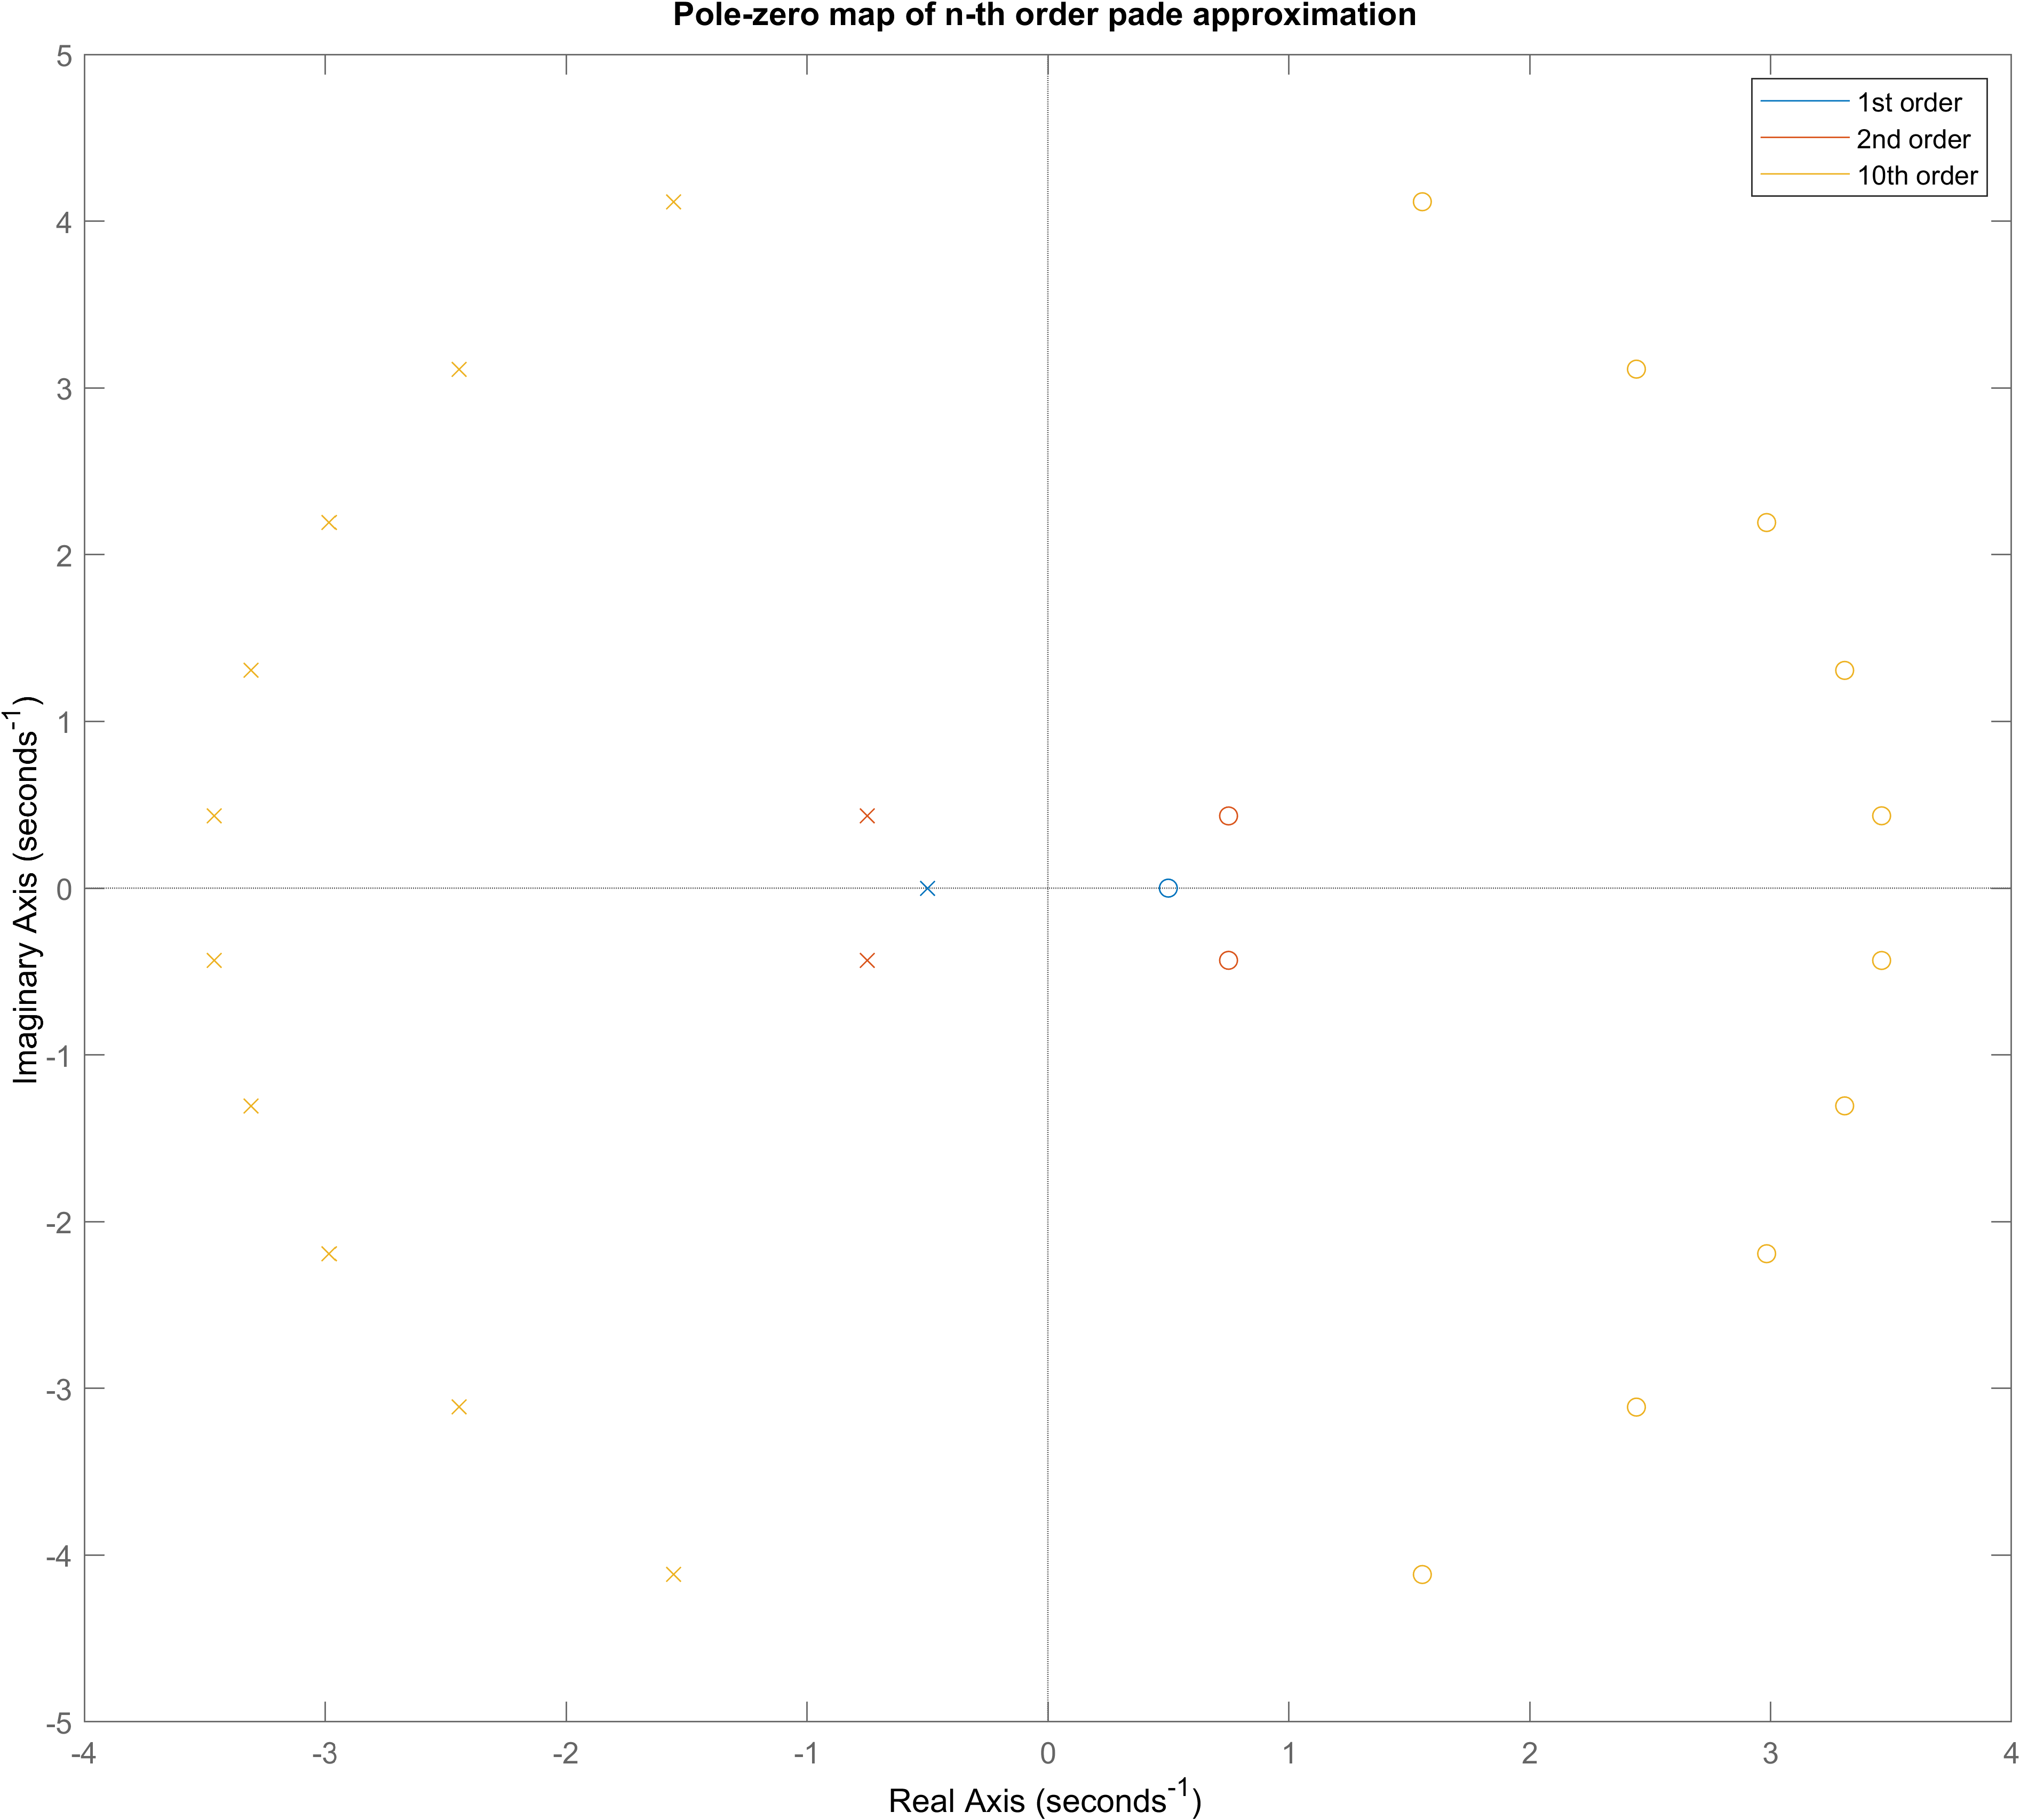
\includegraphics[width=0.8\textwidth]{Pictures/PadeApprox.png}
	\caption{Pole-zero map of various order Padé approximations of a 4 second delay}
	\label{fig:PadeApprox}
\end{figure}

An investigation has been performed to show the error in closed-loop pole locations introduced by using a low order approximation. \cref{fig:CLPoles} and \cref{fig:CLPolesZoom} show the closed-loop pole locations when using a $1$st, $2$nd, and $10$th order Padé approximation. The plots show a noticeable difference from $1$st to $2$nd order, but no significant change beyond that.

\begin{figure}[h!]
	\centering
	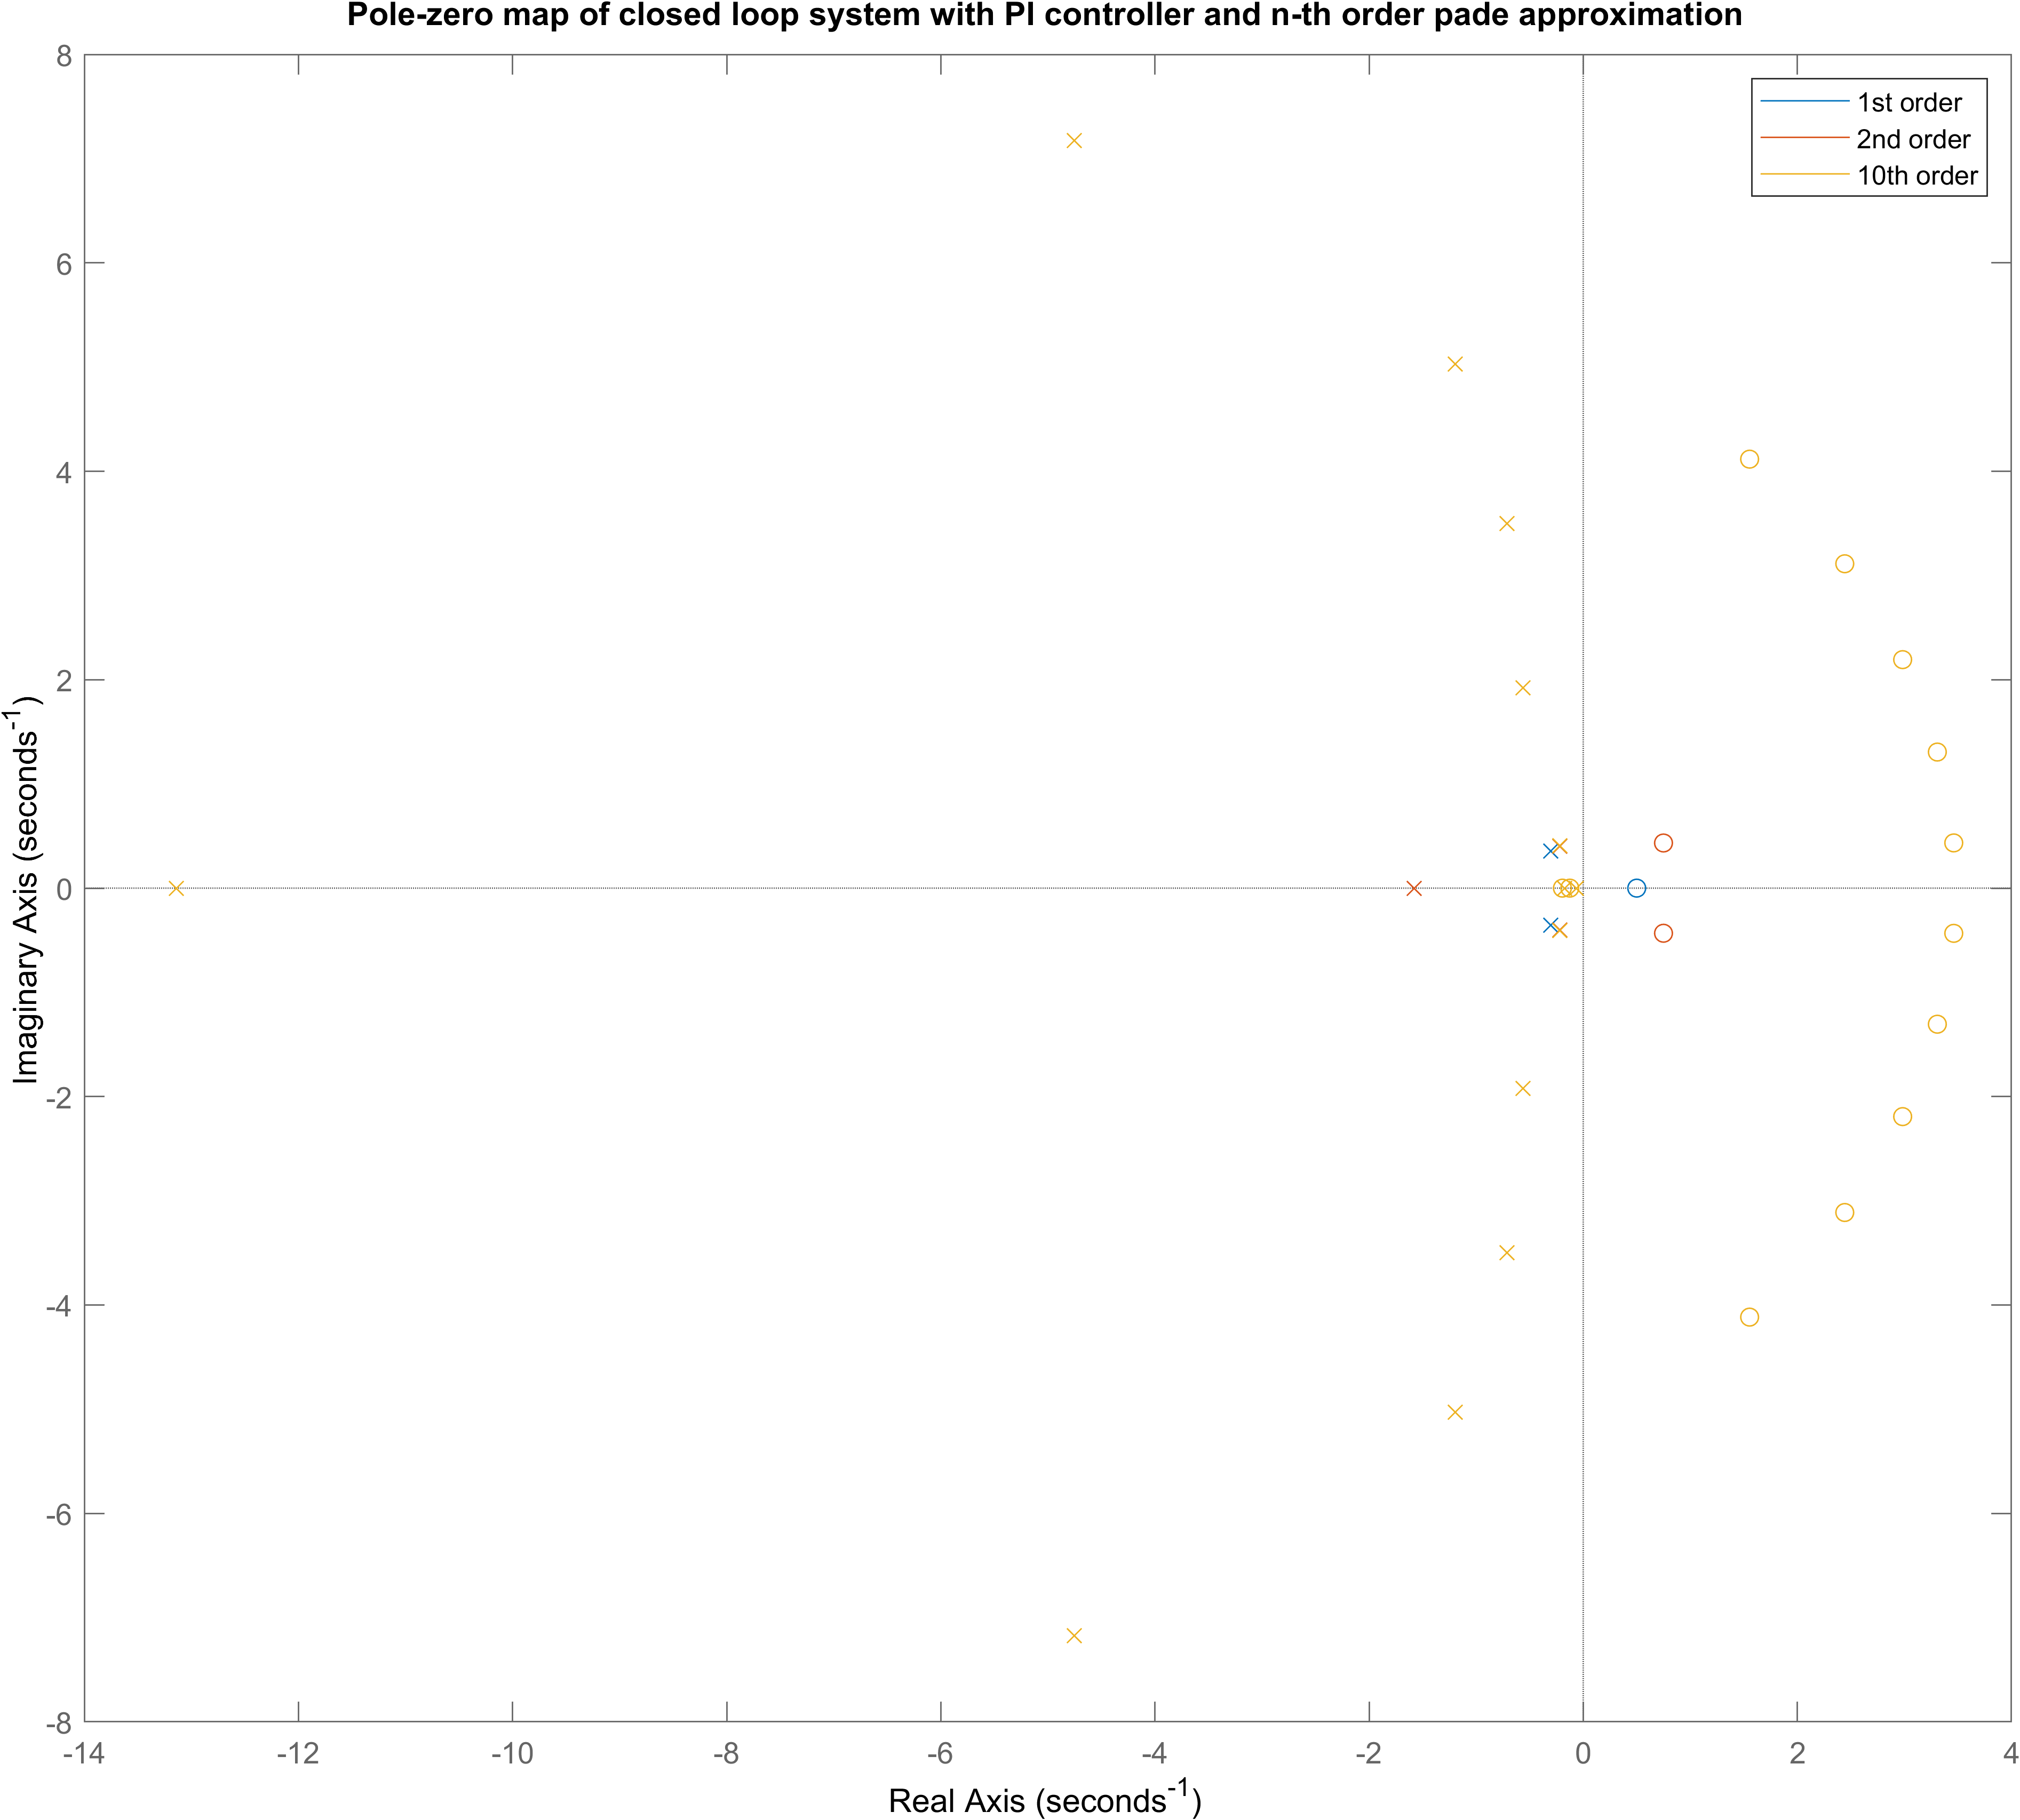
\includegraphics[width=0.8\textwidth]{Pictures/PZmap_CL.png}
	\caption{Pole-zero map of closed-loop pole locations with various order Padé approximations of a 4 second delay}
	\label{fig:CLPoles}
\end{figure}
\begin{figure}[h!]
	\centering
	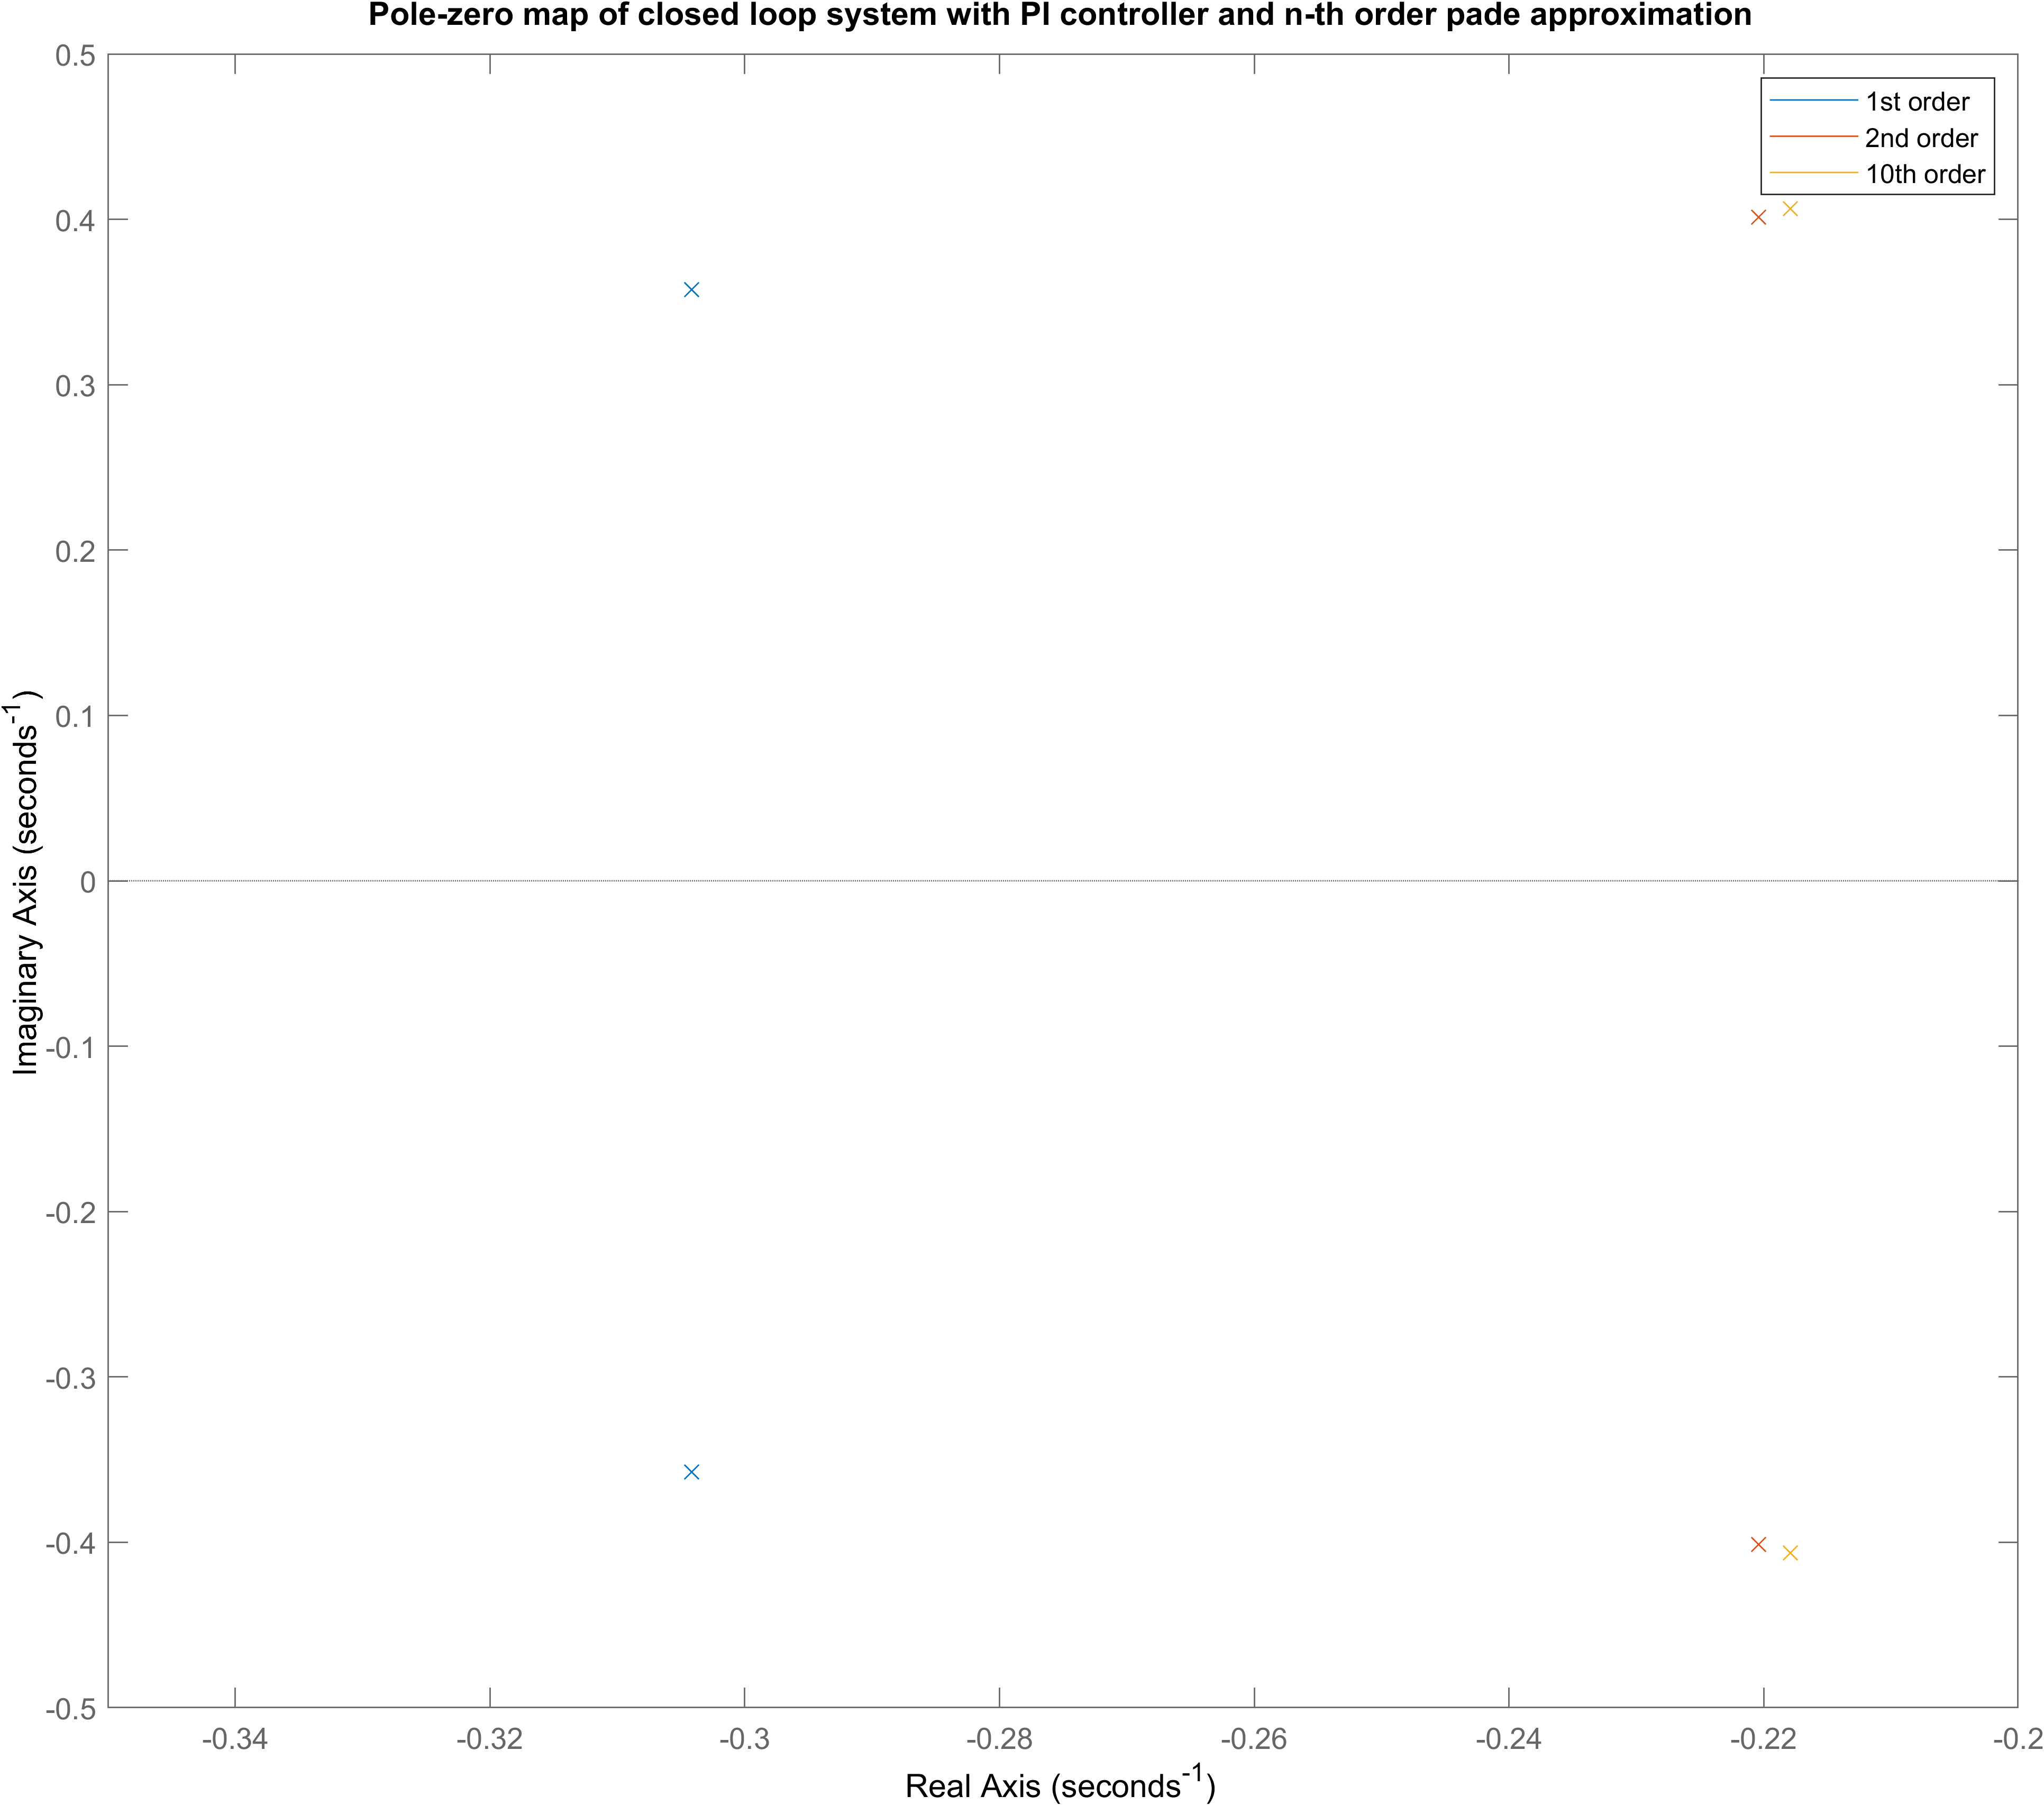
\includegraphics[width=0.8\textwidth]{Pictures/PZmap_CL_zoom.png}
	\caption{Pole-zero map of closed-loop pole locations with various order Padé approximations of a 4 second delay. Zoomed in on the dominant complex conjugate pole pair.}
	\label{fig:CLPolesZoom}
\end{figure}
When considering both convenience of use and modelling error the optimal approximation order was chosen to be 2.

\clearpage

\subsubsection{Requirements for Control Performance}
Before starting the actual root locus design of the controller, the desired performance of the controlled system needs to be defined. \\
The first priority of the controlled system is for it to be stable. This is achieved by ensuring that the closed-loop poles of the system are placed in the left half plane on the s-plane, in accordance with the Routh-Hurwitz criterion. Simultaneously, the inner loop of the system should be at least 5 times faster than the slow outer system. The desired BW of the inner loop is chosen to be $0.1 \si{\frac{rad}{s}}$. This in turn is another restriction on the closed-loop pole locations.

Next, the controlled system should have no steady state error for step inputs. This ensures that the outer controller freely can set and achieve the desired pump flow reference. Lastly the system should have no overshoot and low amount of oscilations in its stepresponse, to indicate a sound phase margin to accommodate model uncertainty.

Since the transfer function of the desired subsystem can be simplified as having two real poles and one zero, and the Padé approximation adds two complex poles and zeros, the system can not be described as a second order system. Therefore traditional requirements like damping ratio do not apply in the normal sense. The requirements will thus be simpler, allowing more freedom for the designer to tune the controller based on the actual stepresponse.

The requirements for the controller can be condensed to the following: 
\begin{itemize}
	\item No poles may be in the right half-plane.
	\item An open-loop pole must be placed in the origin.
	\item The closed-loop system must have a bandwidth of approximately $0.1 \si{\frac{rad}{s}}$.
	\item The closed-loop system must have a time constant of approximately $\frac{1}{BW} = \frac{1}{0.1} = 10 \si{s}$.
\end{itemize}



\subsubsection{Choice of Controller Type}
A PI controller is considered to be a sufficient solution for the requirements put forth. The internal model principle ensures that integral action will take care of the steady state error, and the gain and zero location can be chosen based on the design criteria.

\subsubsection{Root Locus Design}
Since the controller is to be used locally for one pump, the root locus is drawn for the transfer function that takes the rotational speed of pump $1$ as input and the resulting flow of pump $1$ as output. The transfer function is in reduced form, where close pole-zero pairs have been cancelled out. The $2$nd order Padé approximation of a $4$-second time delay is included.


The controller design is then performed in four steps:
\begin{enumerate}
	\item Place one pole at the origin.
	\item Place one real zero in the left half plane.
	\item Select a gain K that yields optimal closed-loop poles.
	\item Evaluate the step response and readjust the zero location and gain value if needed.
\end{enumerate}

While step $1$ requires no intuition, step $2$ has to be done rather carefully. Placing the zero too close to the origin will slow down the integration drastically. Placing it too far to the left, however, creates a locus where the possible closed-loop poles are all undesirable. For step $3$, the gain was increased until the bandwidth of $0.1 \si{\frac{rad}{s}}$ was achieved with no oscillations. As step $4$ implies, the PI controller was designed after some iterations, resulting in the following controller:

 \begin{equation}\label{eq:PITransferFunction}
	G_{PI} = 1.8 \frac{s+0.125}{s}
\end{equation}

With this controller the root locus can be seen on \cref{fig:RootLocus_PadeTwo}. The plot shows zeroes as o's, poles as x's and closed-loop poles as red dots.
\begin{figure}[h!]
	\centering
	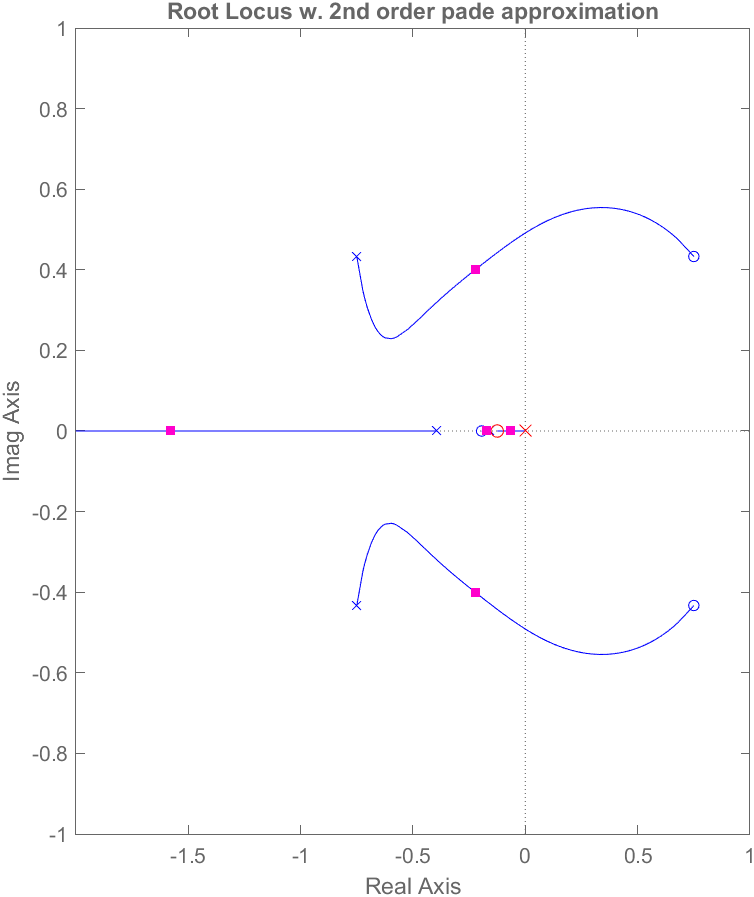
\includegraphics[width=0.8\textwidth]{Pictures/RootLocus_Pade2.png}
	
	\caption{Root locus of delayed pump transfer function with PI controller}
	\label{fig:RootLocus_PadeTwo}
\end{figure}

The resulting closed-loop step response is seen on \cref{fig:StepResponse_Pade2}. The step response shows an initial undershoot. This is not a result of the physical system, but rather the Padé approximation, which places zeroes in the right half plane. These zeroes cause the step response to undershoot in an attempt to delay the signal. Increasing the order of approximation can reduce this, as shown in \cref{fig:StepResponse_Pade10}. \cref{fig:StepResponse_Pade10} also shows that no significant error in the step response is caused by using a $2$nd order approximation rather that $10$th order.

\begin{figure}[h!]
	\centering
	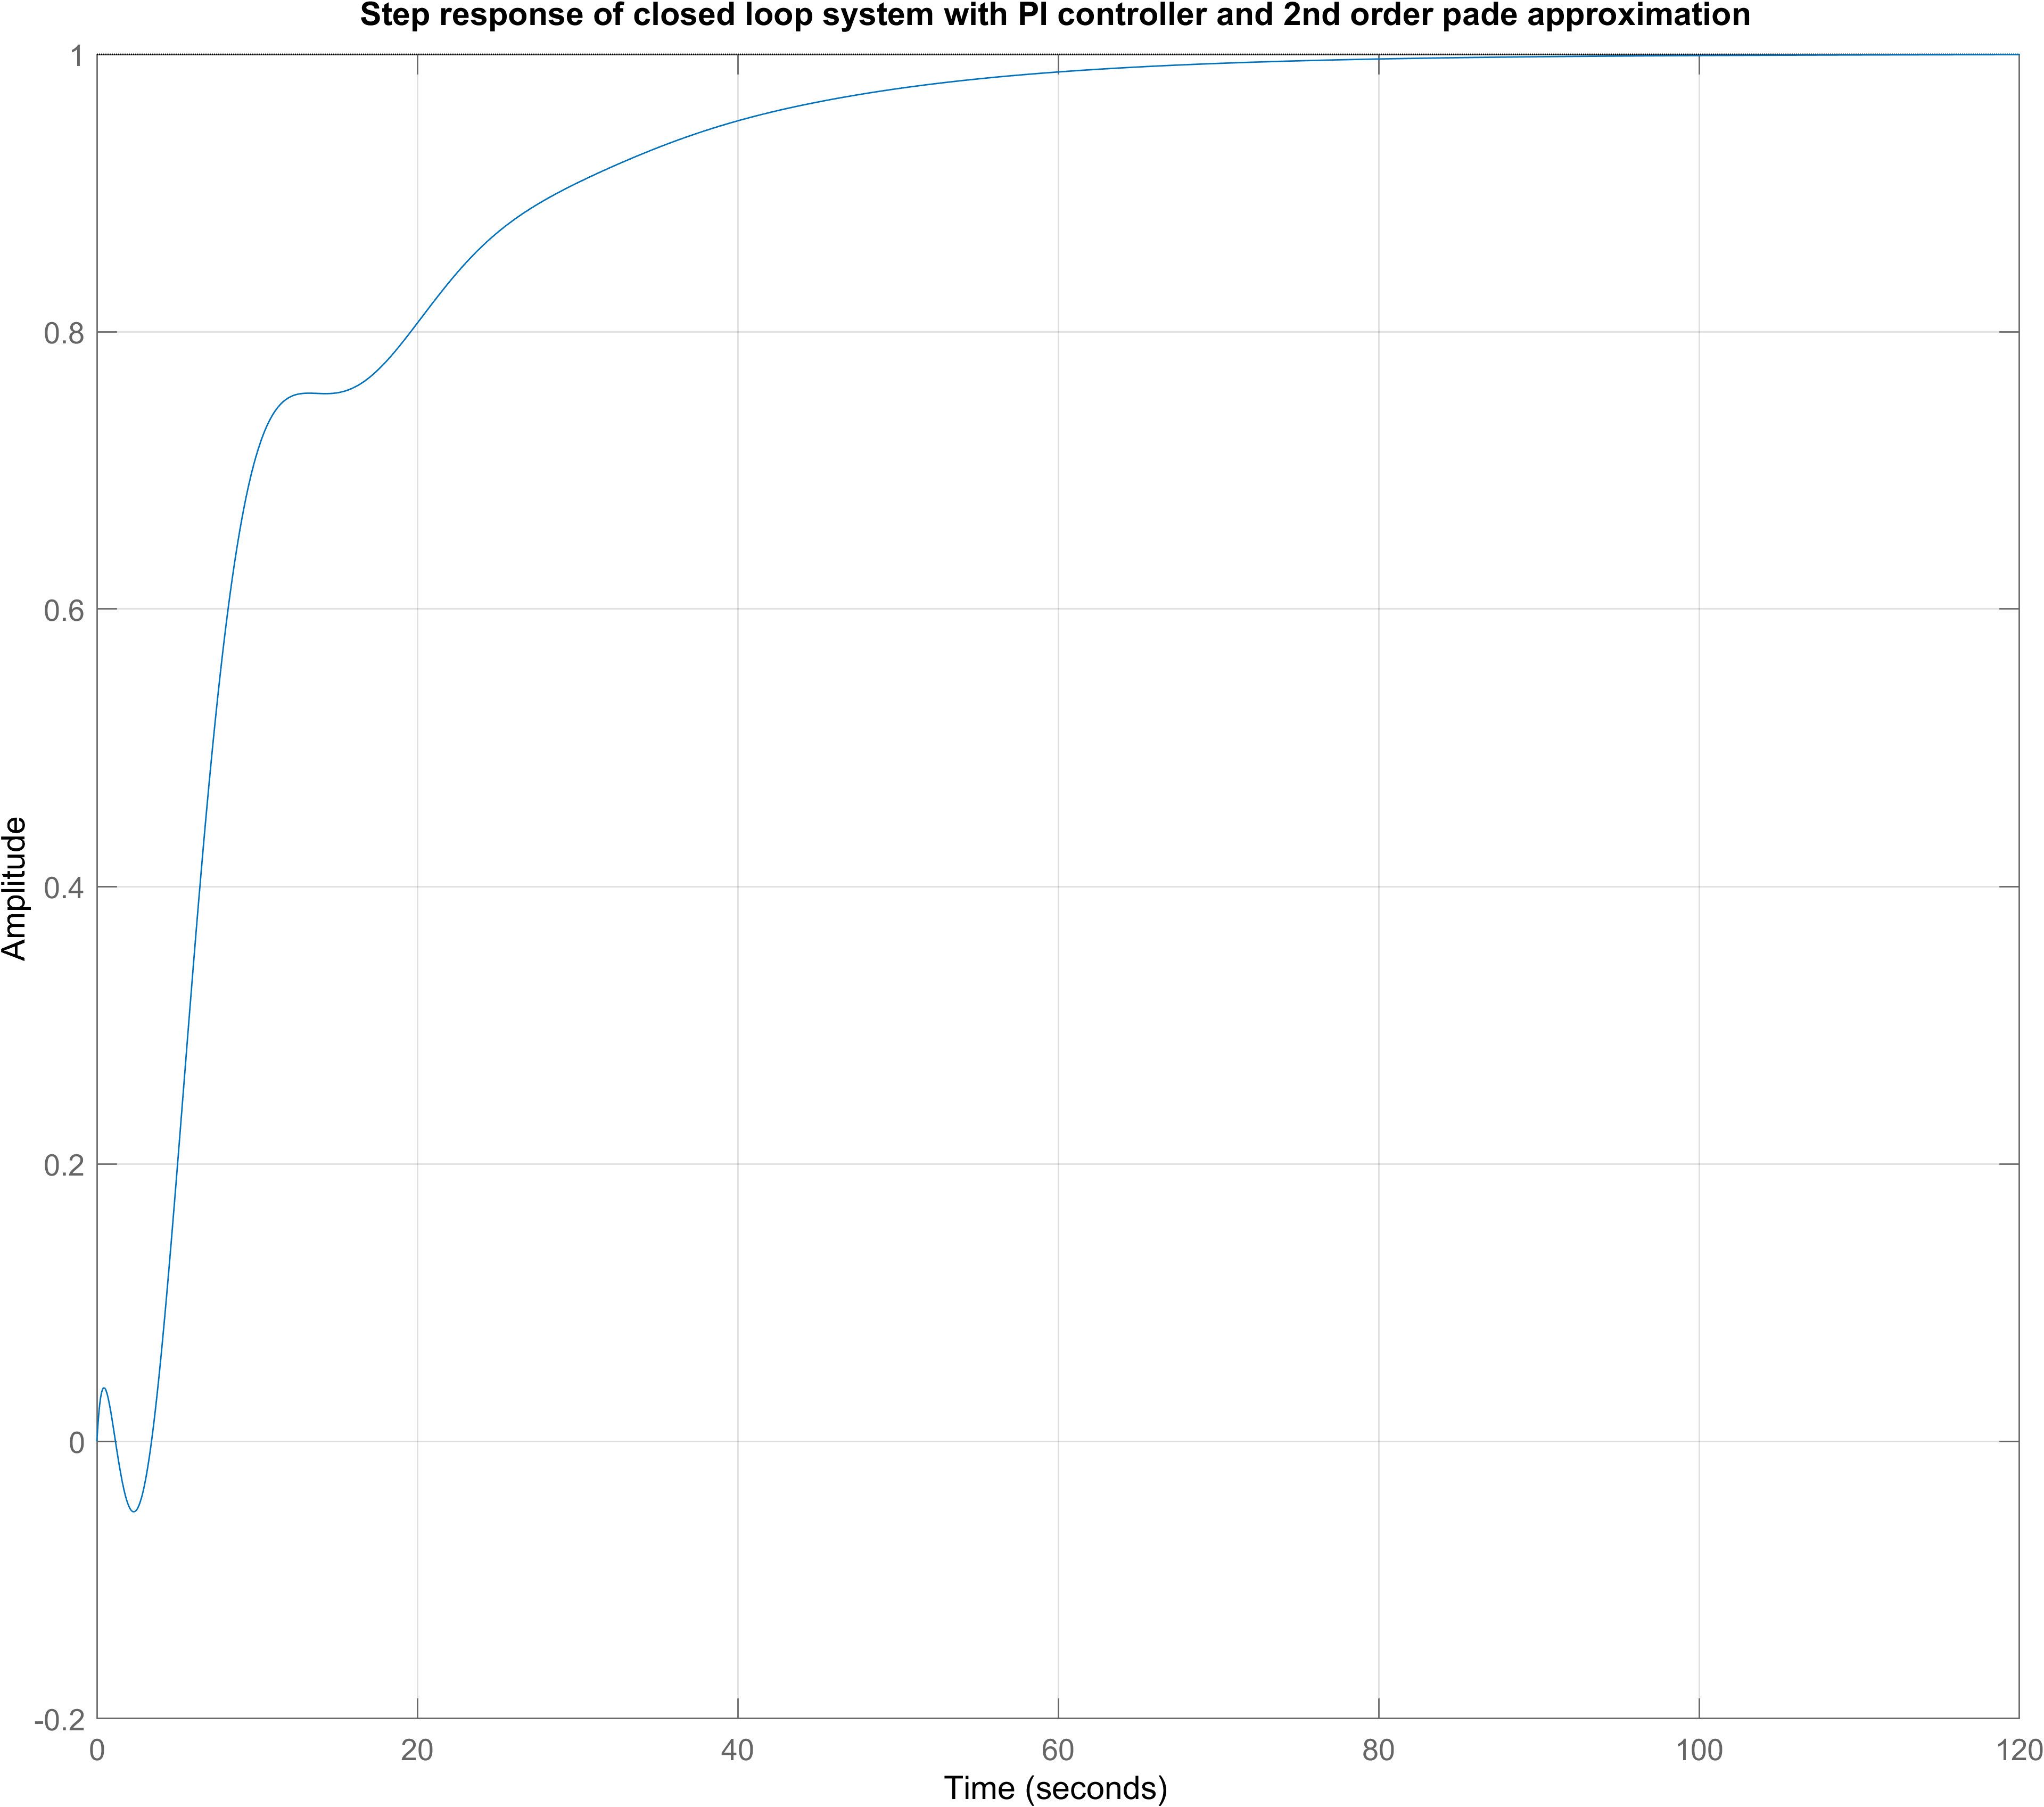
\includegraphics[width=0.8\textwidth]{Pictures/StepResponse_Pade2.png}
	
	\caption{Step response of the closed-loop system with a $2$nd order Padé approximation}
	\label{fig:StepResponse_Pade2}
\end{figure}


\begin{figure}[h!]
	\centering
	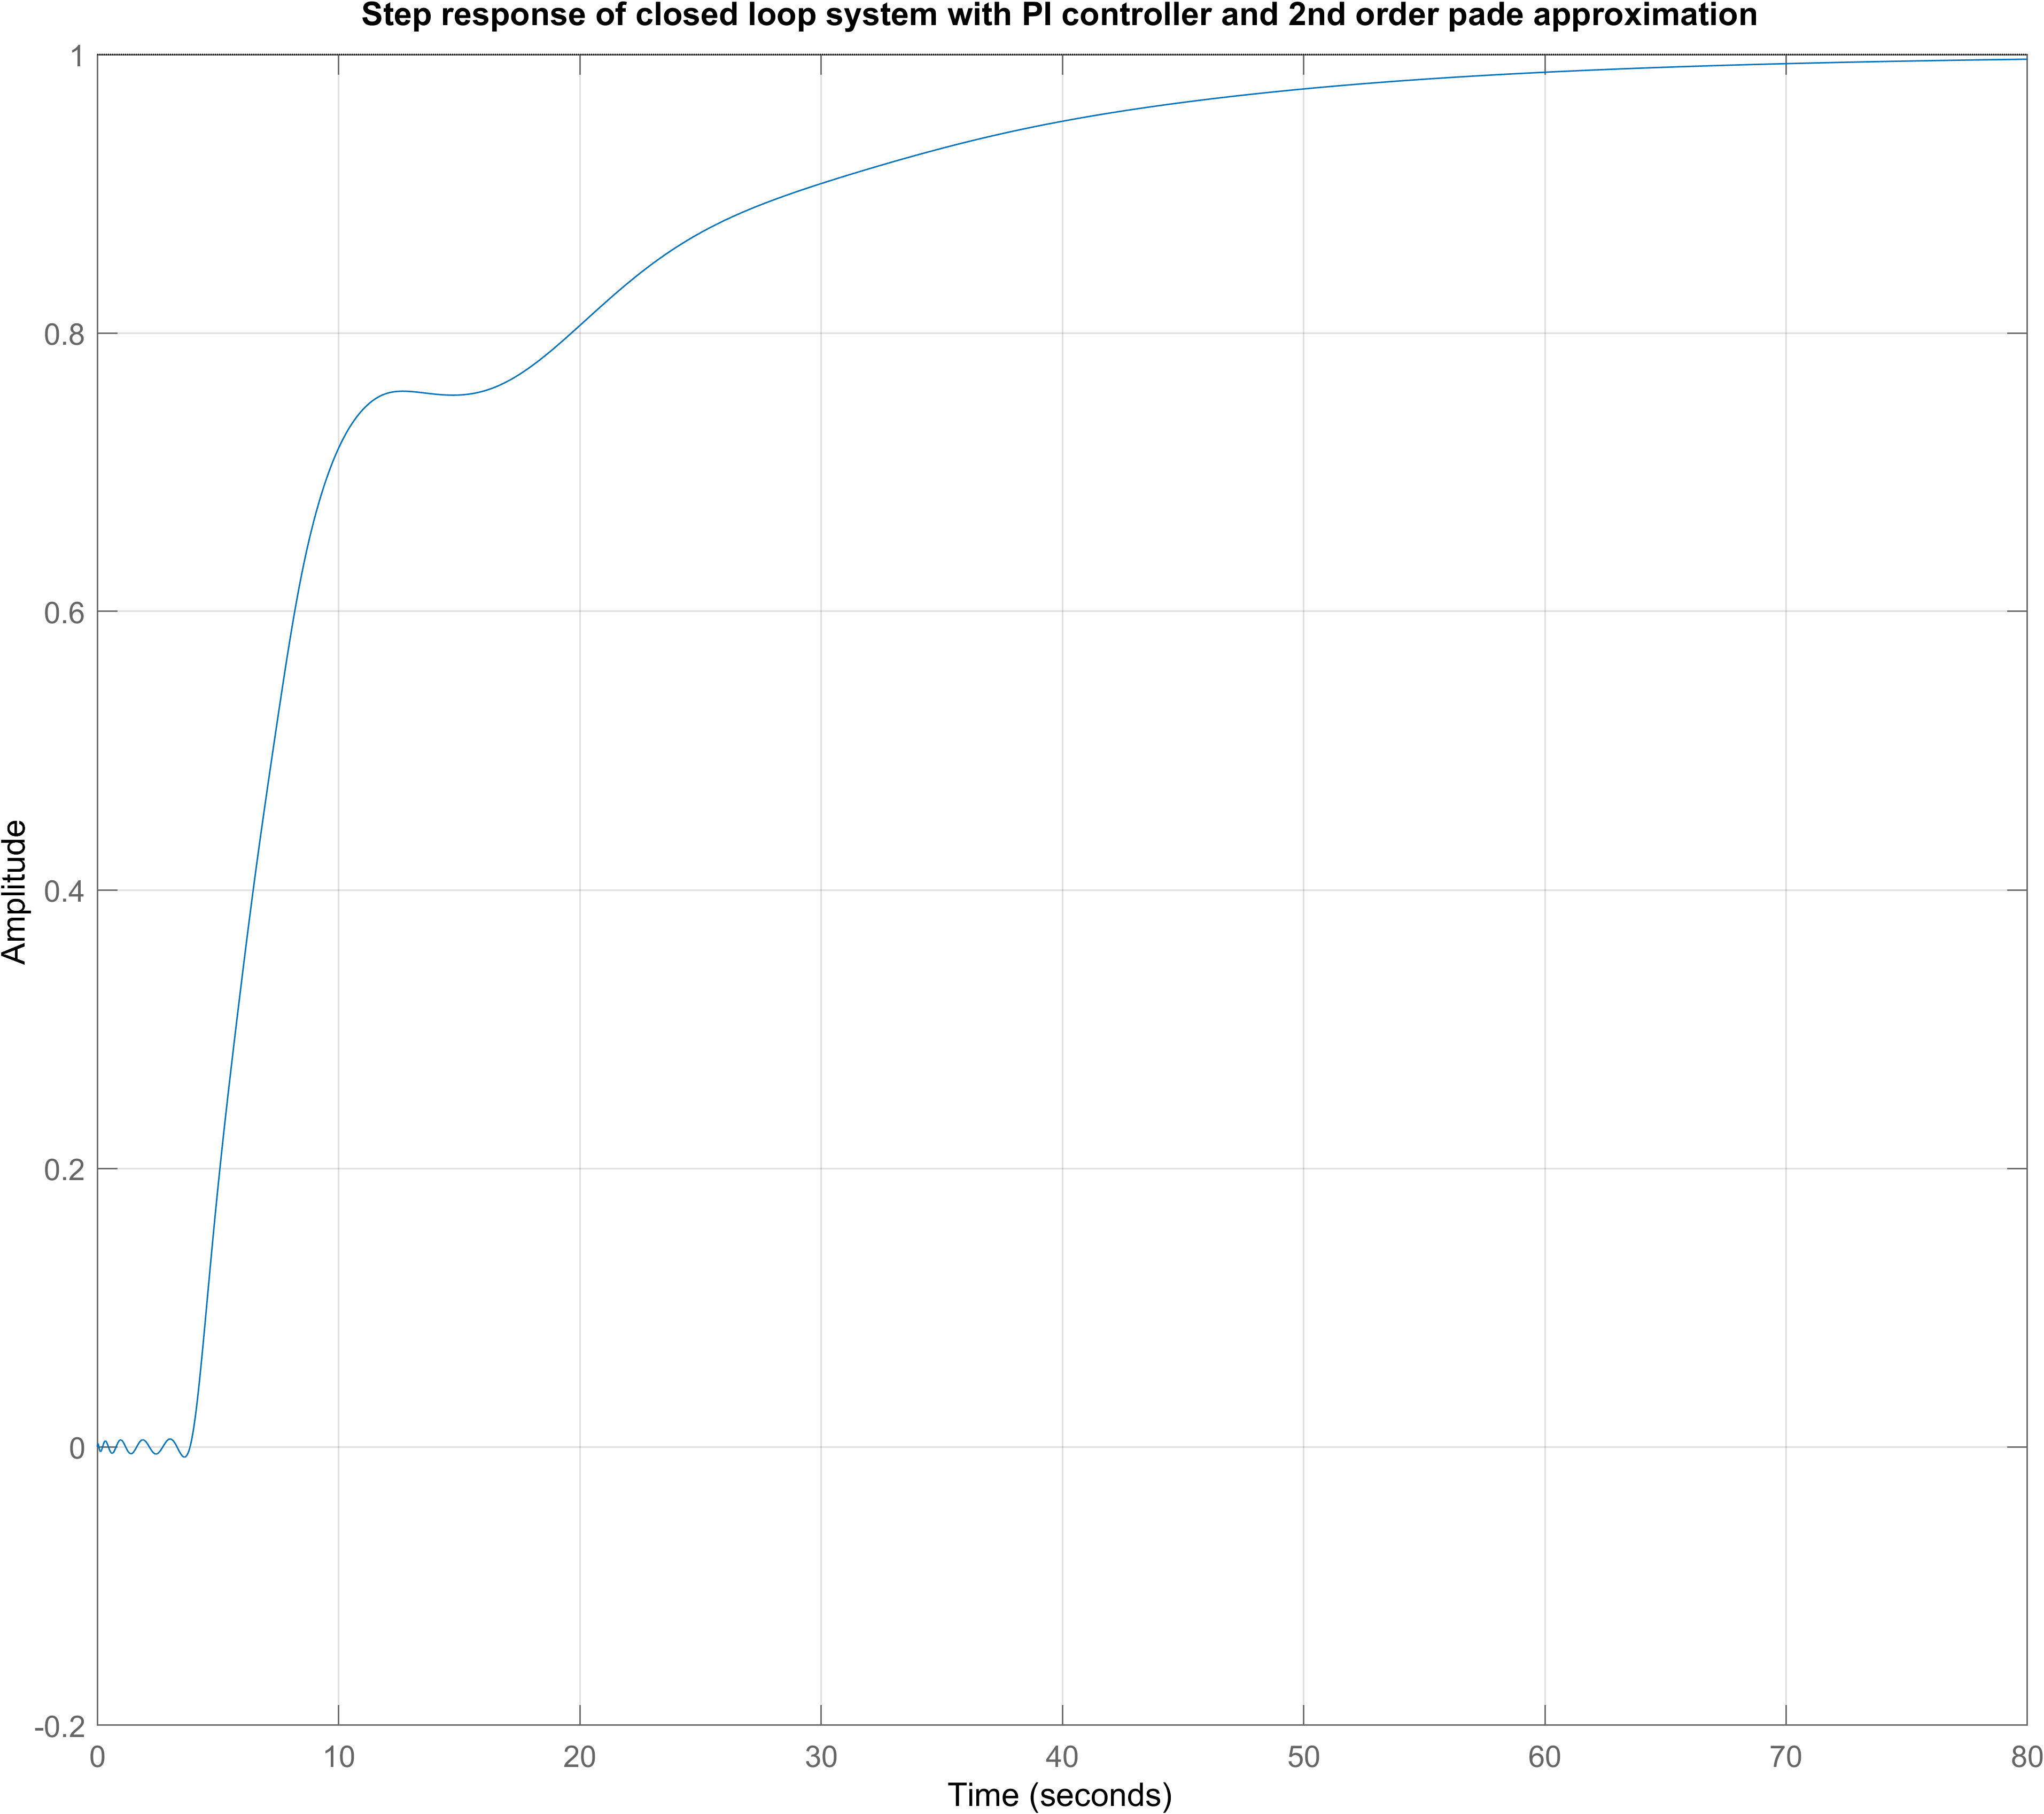
\includegraphics[width=0.8\textwidth]{Pictures/StepResponse_Pade10.png}
	
	\caption{Step response of the closed-loop system with a $10$th order Padé approximation}
	\label{fig:StepResponse_Pade10}
\end{figure}


